\documentclass[12pt,a4paper]{article}

\usepackage[a4paper,margin=2.2cm]{geometry}
\usepackage{fontspec}
\usepackage{polyglossia}

\setmainlanguage{vietnamese}

\setmainfont{TeX Gyre Termes}
\setsansfont{TeX Gyre Heros}
\usepackage{graphicx}
\usepackage{booktabs}
\usepackage{longtable}
\usepackage{array}
\usepackage{xcolor}
\usepackage{hyperref}
\usepackage{float}
\usepackage{caption}
\usepackage{enumitem}
\usepackage{titlesec}
\usepackage{fancyhdr}
\usepackage{lastpage}

\hypersetup{
  colorlinks=true,
  linkcolor=blue!50!black,
  urlcolor=blue!50!black,
  citecolor=blue!50!black
}

\definecolor{FinOpsBlue}{HTML}{124F7A}
\definecolor{FinOpsGreen}{HTML}{1F7A5C}
\definecolor{FinOpsGray}{HTML}{5B6670}
\definecolor{LightBox}{HTML}{F4F8FA}

\titleformat{\section}
  {\Large\bfseries\color{FinOpsBlue}}
  {\thesection}{0.8em}{}
\titleformat{\subsection}
  {\large\bfseries\color{FinOpsGreen}}
  {\thesubsection}{0.8em}{}

\pagestyle{fancy}
\fancyhf{}
\lhead{Day 25 - GPU FinOps}
\rhead{Le Huy Hong Nhat}
\cfoot{\thepage/\pageref{LastPage}}

\setlist[itemize]{leftmargin=1.6em,itemsep=0.25em}
\renewcommand{\arraystretch}{1.25}

\newcommand{\metric}[2]{\textbf{#1} & #2 \\}

\title{
  \vspace{-1.5cm}
  \textbf{\Huge Báo Cáo GPU FinOps}\\
  \vspace{0.3cm}
  \Large Day 25 - GPU FinOps \& Cost Optimization
}
\author{Le Huy Hong Nhat \\ MSSV: 2A202600099}
\date{13/05/2026}

\linespread{1.15}
\begin{document}
\maketitle
\thispagestyle{empty}

\begin{center}
\colorbox{LightBox}{
  \begin{minipage}{0.92\textwidth}
  \textbf{Tóm tắt kết quả.}
  Mock GPU platform được chạy bằng Docker Compose local và notebook Kaggle gọi API qua tunnel.
  Real GPU training chạy trên Tesla T4. AMP nhanh hơn FP32 2.11x và giảm chi phí 52.7\%.
  Advanced analysis cho thấy expected project cost là \$4261.44 và roadmap optimization có thể tiết kiệm 87.8\%.
  \end{minipage}
}
\end{center}

\vspace{0.5cm}
\tableofcontents
\newpage

\section{Giới thiệu}

\subsection{Mục tiêu của bài lab}

Bài lab xây dựng một quy trình GPU FinOps end-to-end, bao gồm quan sát tài nguyên GPU,
ghi nhận billing theo workload, mô phỏng spot/preemptible instances, đánh giá autoscaling,
phân tích waste và tối ưu chi phí thông qua mixed precision, scheduling, spot instances
và capacity planning.

Mục tiêu cụ thể:
\begin{itemize}
  \item Theo dõi trạng thái GPU cluster: node count, busy/idle GPUs, utilization, memory và power draw.
  \item Gắn workload với billing record để hiểu chi phí theo từng job/project.
  \item Mô phỏng spot instances và preemption để đánh giá savings/risk trade-off.
  \item Dùng autoscaling policy để phản ứng với utilization threshold.
  \item Đo real GPU training trên Tesla T4 và so sánh FP32 với Mixed Precision AMP.
  \item Xây dựng advanced cost forecast, optimization roadmap và budget decision.
\end{itemize}

\subsection{Tổng quan về GPU FinOps}

GPU FinOps là thực hành quản trị chi phí GPU dựa trên dữ liệu vận hành.
Điểm cốt lõi không chỉ là giảm giá mỗi giờ GPU, mà là tối ưu toàn bộ cost-performance:
tăng utilization, giảm idle waste, chọn đúng GPU type, dùng spot cho workload chịu được
preemption, và đo chi phí theo workload thay vì chỉ nhìn tổng hóa đơn.

Trong bài lab này, kiến trúc gồm hai phần:
\begin{itemize}
  \item \textbf{Local Docker services}: gateway, gpu-node-manager, billing-api, spot-manager, autoscaler và cost-tracker.
  \item \textbf{Remote notebook trên Kaggle}: chạy experiment, gọi local gateway qua tunnel và thực hiện real GPU training.
\end{itemize}

\section{Phân tích từng phần}

\subsection{Part 1-7: Mock cluster analysis}

\subsubsection*{Cluster monitoring insights}

Mock cluster ban đầu có 9 nodes với 18 GPUs. Trong snapshot monitoring:

\begin{table}[H]
\centering
\begin{tabular}{ll}
\toprule
\textbf{Metric} & \textbf{Giá trị} \\
\midrule
\metric{Total GPUs}{18}
\metric{Busy GPUs}{13}
\metric{Idle GPUs}{5}
\metric{Average utilization}{56.7\%}
\metric{Memory used / capacity}{252.1 GB / 448.0 GB}
\metric{Total power draw}{1417 W}
\metric{Node count}{9}
\bottomrule
\end{tabular}
\caption{Cluster metrics ban đầu.}
\end{table}

Kết quả này cho thấy cluster đang có workload thật sự, nhưng vẫn còn idle capacity.
Sau khi submit thêm workloads, cluster đạt 18/18 GPUs busy với utilization 79.2\%.
Điều này tạo đủ áp lực để kiểm thử autoscaling policy.

\subsubsection*{Cost tracking observations}

Billing summary sau workload submission:

\begin{table}[H]
\centering
\begin{tabular}{ll}
\toprule
\textbf{Metric} & \textbf{Giá trị} \\
\midrule
\metric{Total cost}{\$5.2869}
\metric{Total savings}{\$5.5380}
\metric{Budget used}{5.3\%}
\metric{Alert status}{OK}
\bottomrule
\end{tabular}
\caption{Billing summary của mock workload.}
\end{table}

Cost tracker ghi nhận 5 snapshots với mỗi interval có total cost \$0.049722,
idle cost \$0.001944 và waste 3.9\%. Waste report tổng hợp cho thấy average waste 4.1\%,
severity LOW, nhưng potential monthly saving lên đến \$503.88. Điều này minh họa một nguyên tắc
quan trọng của GPU FinOps: idle waste nhỏ theo từng interval vẫn có thể thành chi phí lớn nếu kéo dài.

\begin{figure}[H]
\centering
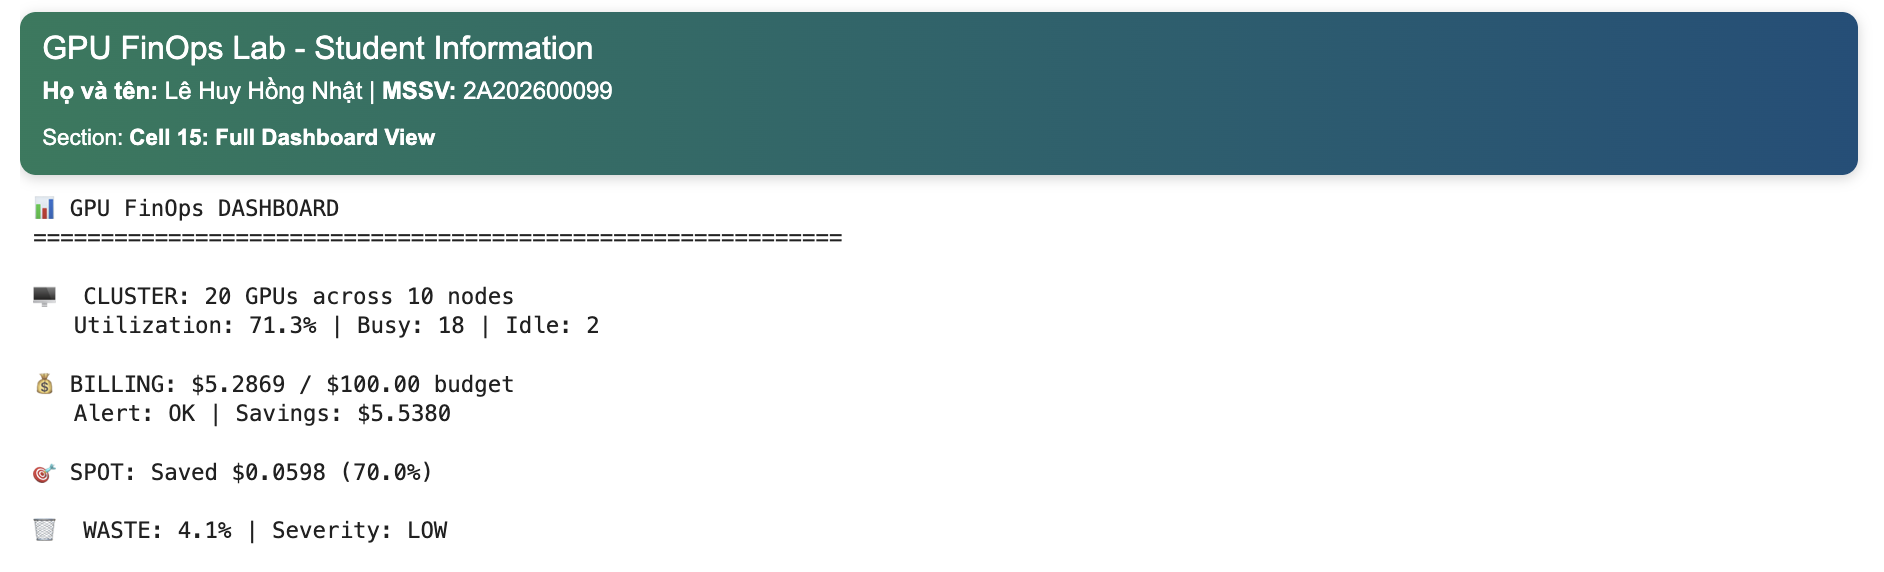
\includegraphics[width=0.95\textwidth]{screenshots/part5_dashboard.png}
\caption{Mock FinOps dashboard: cluster, billing, spot và waste.}
\end{figure}

\begin{figure}[H]
\centering

\includegraphics[width=0.95\textwidth]{screenshots/generated_charts/finops_timeseries.png}
\caption{Time-series cost tracking: active cost, idle cost và waste percentage.}
\end{figure}

\subsubsection*{Spot instance savings analysis}

Spot pricing và preemption workflow cho kết quả:

\begin{table}[H]
\centering
\begin{tabular}{ll}
\toprule
\textbf{Metric} & \textbf{Giá trị} \\
\midrule
\metric{T4 spot price}{\$0.2500/hr}
\metric{A100 spot price}{\$2.8853/hr}
\metric{V100 spot price}{\$1.5778/hr}
\metric{Spot requests}{3 requests granted}
\metric{Preemption event}{1 instance preempted, 5 still active}
\metric{Spot cost}{\$0.0167}
\metric{On-demand equivalent}{\$0.0557}
\metric{Savings}{\$0.0390 (70.0\%)}
\bottomrule
\end{tabular}
\caption{Spot/preemptible savings analysis.}
\end{table}

Spot instances tiết kiệm lớn nhưng có rủi ro preemption.
Vì vậy chiến lược hợp lý là dùng spot cho batch job, training có checkpoint hoặc workload retryable;
không nên dùng mặc định cho workload latency-critical hoặc không chịu được interruption.

\subsubsection*{Autoscaling behavior}

Autoscaling policy được update với scale-up threshold 70.0\%, scale-down threshold 25.0\%,
cooldown 30 giây, min nodes 2 và max nodes 10. Khi utilization đạt 79.2\%, autoscaler quyết định
\texttt{SCALE\_UP}, tăng cluster từ 9 lên 10 nodes. Sau đó 5 evaluation cycles đều \texttt{no\_action}
với utilization 71.3\%, nodes 10 -> 10.

Kết quả này cho thấy autoscaler hoạt động đúng theo threshold, nhưng cũng chỉ ra một điểm cần quản trị:
threshold phải được cân bằng để tránh scale-up quá nhanh gây tăng cost hoặc scale-down quá mạnh gây queue workload.

\subsubsection*{Waste analysis và recommendations}

Waste report:
\begin{itemize}
  \item Average waste: 4.1\%.
  \item Total idle cost: \$0.019440.
  \item Total cost: \$0.479720.
  \item Potential monthly save: \$503.88.
  \item Severity: LOW.
\end{itemize}

Recommendations gồm:
\begin{itemize}
  \item \textbf{USE\_SPOT}: chuyển workload fault-tolerant sang spot instances để tiết kiệm 60-70\%.
  \item \textbf{SCHEDULING}: chạy job không gấp trong off-peak hours để tận dụng spot price thấp hơn.
\end{itemize}

Complete workflow cuối cùng ghi nhận total spend \$5.4560, total saved \$5.6604,
budget usage 5.5\% và alert OK.

\begin{figure}[H]
\centering
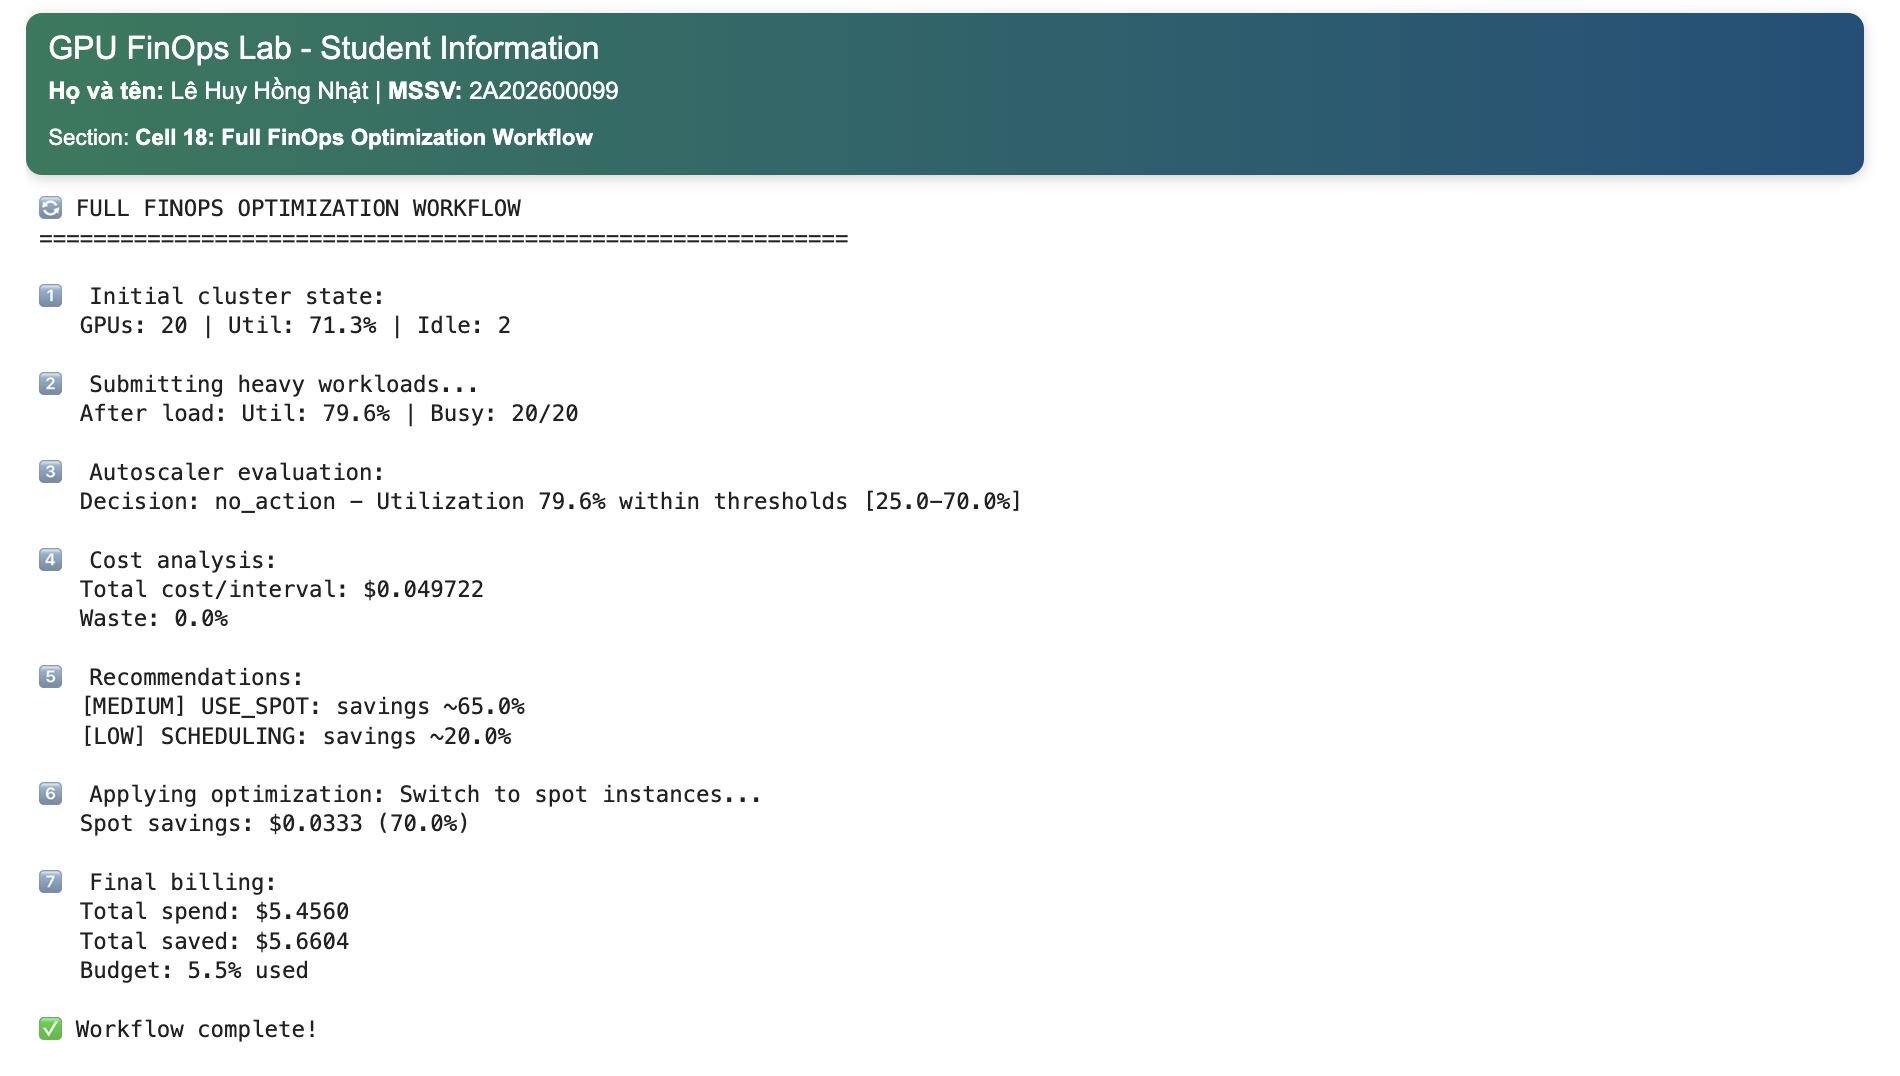
\includegraphics[width=0.95\textwidth]{screenshots/part7_full_workflow.png}
\caption{Complete FinOps workflow từ monitoring đến final billing.}
\end{figure}

\subsection{Part 8: Real GPU training}

Notebook chạy real GPU trên Tesla T4:

\begin{table}[H]
\centering
\begin{tabular}{ll}
\toprule
\textbf{Metric} & \textbf{Giá trị} \\
\midrule
\metric{GPU}{Tesla T4}
\metric{Memory}{15.6 GB}
\metric{Compute capability}{7.5}
\metric{PyTorch}{2.10.0+cu128}
\metric{CUDA build}{12.8}
\metric{Device}{cuda}
\bottomrule
\end{tabular}
\caption{Thông tin real GPU runtime.}
\end{table}

\subsubsection*{FP32 vs Mixed Precision AMP comparison}

\begin{table}[H]
\centering
\begin{tabular}{lccc}
\toprule
\textbf{Metric} & \textbf{FP32} & \textbf{AMP} & \textbf{Improvement} \\
\midrule
Total time & 117.3s & 55.5s & 2.11x faster \\
Peak memory & 0.82 GB & 0.60 GB & 0.22 GB saved \\
Estimated cost & \$0.011399 & \$0.005392 & \$0.006007 saved \\
Cost saving & -- & -- & 52.7\% \\
Average GPU util & 97.3\% & 95.1\% & high utilization \\
Average power & 67.1W & 66.0W & similar power \\
\bottomrule
\end{tabular}
\caption{So sánh FP32 và Mixed Precision AMP.}
\end{table}

FP32 baseline train 3 epochs với accuracy tăng từ 35.5\% lên 69.1\%.
AMP train 3 epochs với accuracy tăng từ 31.4\% lên 63.6\%.
Trong cùng số epochs, AMP nhanh hơn đáng kể và giảm chi phí 52.7\%.

\subsubsection*{Cost savings achieved}

Extrapolated savings:
\begin{itemize}
  \item 1 ngày training: FP32 \$8.40 vs AMP \$3.97, tiết kiệm \$4.43.
  \item 1 tuần training: FP32 \$58.80 vs AMP \$27.81, tiết kiệm \$30.99.
  \item 1 tháng training: FP32 \$252.00 vs AMP \$119.20, tiết kiệm \$132.80.
\end{itemize}

AMP là chiến lược tối ưu chi phí hiệu quả vì effort thấp, rủi ro thấp và thường không làm giảm chất lượng đáng kể
nếu được kiểm chứng bằng validation metrics.

\subsubsection*{GPU utilization patterns}

Cả FP32 và AMP đều có utilization cao, lần lượt 97.3\% và 95.1\%.
Điều này cho thấy experiment đang dùng GPU hiệu quả và không bị bottleneck nặng ở data loading.
Telemetry cũng ghi nhận power trung bình khoảng 66-67W.

\begin{figure}[H]
\centering

\includegraphics[width=0.95\textwidth]{screenshots/generated_charts/real_gpu_comparison.png}
\caption{FP32 vs AMP: time, cost và utilization/epoch comparison.}
\end{figure}

\begin{figure}[H]
\centering

\includegraphics[width=0.92\textwidth]{screenshots/generated_charts/real_gpu_telemetry.png}
\caption{Real GPU telemetry: utilization, memory, power và temperature.}
\end{figure}

\begin{figure}[H]
\centering

\includegraphics[width=0.85\textwidth]{screenshots/generated_charts/cost_per_epoch.png}
\caption{Cost per epoch giữa FP32 và AMP.}
\end{figure}

\subsection{Part 8.5: Advanced analysis}

\subsubsection*{Multi-GPU scaling efficiency}

Multi-GPU cost analysis cho thấy:
\begin{itemize}
  \item Lowest cost: 1x A100 với cost \$7.34.
  \item Fastest run: 8x A100 với runtime 0.36h.
  \item Best cost/performance: 8x A100 với \$1.87/speedup unit.
\end{itemize}

Kết quả nhấn mạnh rằng scaling không tuyến tính. Thêm GPU giúp giảm runtime nhưng tăng GPU-hour.
Vì vậy cần so sánh theo cost-per-performance, deadline và budget thay vì chỉ chọn cấu hình nhanh nhất.

\begin{figure}[H]
\centering

\includegraphics[width=0.95\textwidth]{screenshots/generated_charts/multi_gpu_scaling.png}
\caption{Multi-GPU cost curve và scaling efficiency.}
\end{figure}

\subsubsection*{Project cost forecasting}

Forecast multi-phase project:

\begin{table}[H]
\centering
\begin{tabular}{ll}
\toprule
\textbf{Metric} & \textbf{Giá trị} \\
\midrule
\metric{Base total}{\$3551.20}
\metric{Contingency}{\$710.24 (20\%)}
\metric{Expected total}{\$4261.44}
\metric{95\% interval}{\$2913.09 - \$5609.79}
\metric{Best / worst case}{\$2578.82 - \$5233.82}
\bottomrule
\end{tabular}
\caption{Project cost forecasting summary.}
\end{table}

Expected total vẫn nằm trong mức kiểm soát, nhưng upper confidence interval có thể vượt \$5600.
Điều này chứng minh cần contingency và confidence interval khi lập budget GPU, đặc biệt cho hyperparameter tuning
hoặc phase có uncertainty cao.

\begin{figure}[H]
\centering

\includegraphics[width=0.95\textwidth]{screenshots/generated_charts/project_forecast.png}
\caption{Project forecast theo phase và scenario.}
\end{figure}

\subsubsection*{Optimization strategy prioritization}

Optimization opportunity analysis bắt đầu từ baseline cost \$1468.00.
Roadmap tối ưu cuối cùng giảm cost xuống \$179.68, tiết kiệm \$1288.32 tương đương 87.8\%.

Các chiến lược quan trọng:
\begin{itemize}
  \item Mixed Precision AMP: low effort, low risk, savings cao.
  \item Optimize Batch Size: cải thiện utilization mà không tăng preemption risk.
  \item Early Stopping: giới hạn runaway training/tuning cost.
  \item Spot Instances: savings lớn nhưng cần checkpoint/retry để kiểm soát risk.
  \item Switch GPU Type: tiềm năng lớn nhưng effort/risk cao hơn.
\end{itemize}

\begin{figure}[H]
\centering

\includegraphics[width=0.95\textwidth]{screenshots/generated_charts/optimization_roadmap.png}
\caption{Optimization priority matrix và cumulative savings roadmap.}
\end{figure}

\begin{figure}[H]
\centering

\includegraphics[width=0.95\textwidth]{screenshots/generated_charts/advanced_finops_dashboard.png}
\caption{Integrated advanced FinOps dashboard.}
\end{figure}

\subsubsection*{Challenge exercise}

Challenge scenario là fine-tuning LLM với baseline 8x A100 trong 200h, FP32, on-demand,
budget \$5000 và deadline 2 tuần. Baseline cost là \$5872.00, vượt budget.

Chiến lược được chọn:
\begin{itemize}
  \item GPU plan: 8x A100.
  \item Runtime sau scaling analysis: 35.7h, nhỏ hơn deadline 336h.
  \item Raw GPU cost: \$1048.57.
  \item Forecast before strategy: \$1215.52.
  \item Strategy savings: 61.8\%.
  \item Final expected cost: \$464.94.
  \item 95\% interval after optimization: \$307.71 - \$622.16.
  \item Verdict: UNDER BUDGET.
\end{itemize}

\begin{figure}[H]
\centering
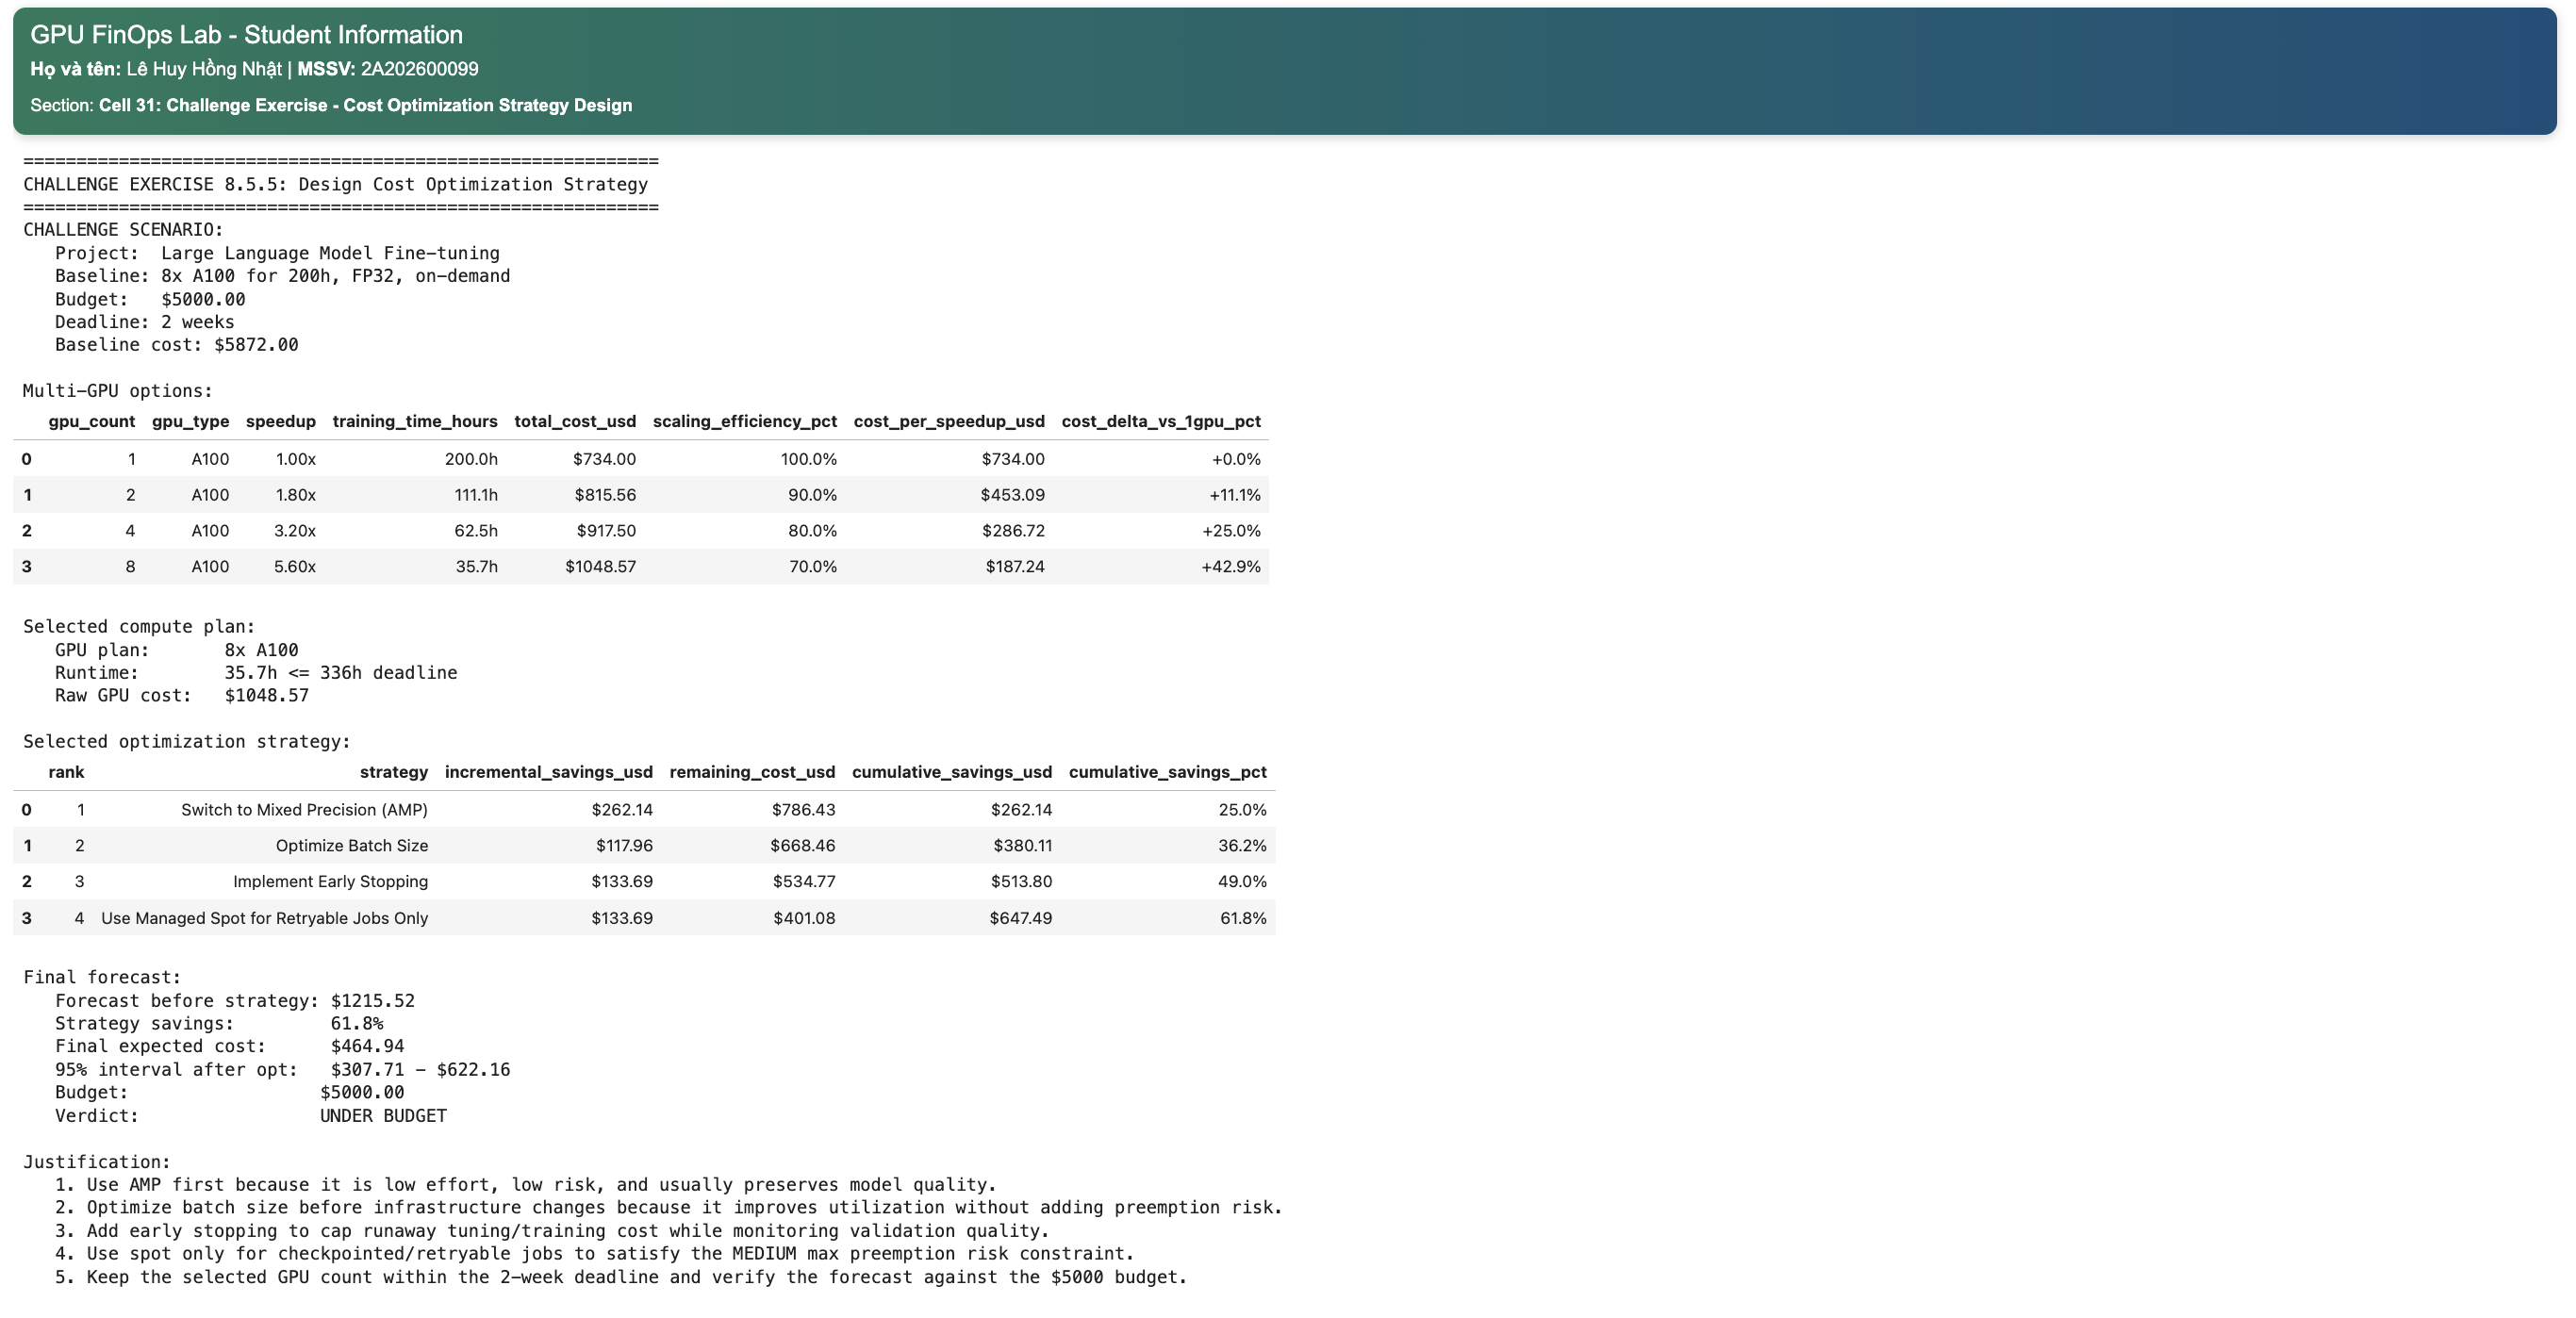
\includegraphics[width=0.95\textwidth]{screenshots/part85_challenge_strategy.png}
\caption{Challenge strategy: forecast, budget verdict và justification.}
\end{figure}

\section{Kết luận và học hỏi}

\subsection{Những kỹ năng FinOps đã học}

\begin{itemize}
  \item Đo GPU utilization, memory, power và idle waste để hiểu chi phí thật của GPU platform.
  \item Gắn workload execution với billing record để tính cost theo project/workload.
  \item Đánh giá spot/preemptible savings song song với rủi ro preemption.
  \item Dùng autoscaling policy để giảm over-provisioning và phản ứng với demand.
  \item So sánh FP32 và AMP theo performance, memory, utilization và USD cost.
  \item Forecast project cost với uncertainty và contingency thay vì chỉ dùng base cost.
\end{itemize}

\subsection{Các chiến lược cost optimization hiệu quả}

\begin{itemize}
  \item \textbf{Mixed Precision AMP}: nhanh hơn 2.11x và tiết kiệm 52.7\% cost trong experiment thực tế.
  \item \textbf{Spot instances}: tiết kiệm 70.0\% trong mock workflow khi dùng cho workload phù hợp.
  \item \textbf{Autoscaling}: scale-up khi utilization vượt threshold và tránh giữ quá nhiều idle GPU.
  \item \textbf{Waste monitoring}: idle waste 4.1\% vẫn có thể quy đổi thành monthly savings đáng kể.
  \item \textbf{Optimization roadmap}: kết hợp nhiều chiến lược cho savings tích lũy 87.8\%.
\end{itemize}

\subsection{Ứng dụng thực tế trong projects}

Trong project thực tế, workflow này có thể triển khai thành dashboard FinOps liên tục.
Mỗi training job nên ghi nhận GPU type, runtime, precision mode, cost, utilization và project owner.
Platform team có thể đặt policy: dùng AMP mặc định nếu validation quality không giảm,
dùng spot cho job checkpointed/retryable, đặt budget alert theo project và review định kỳ các workload
có utilization thấp hoặc idle cost cao.

Bài lab cũng cho thấy quyết định GPU không nên chỉ dựa vào tốc độ.
Cấu hình nhiều GPU cần được so sánh bằng cost-per-performance và confidence interval.
Khi deadline lỏng, cấu hình rẻ hơn có thể tốt hơn; khi deadline gấp, cấu hình nhanh hơn vẫn hợp lý
nếu forecast nằm trong budget.

\end{document}
